\begin{comment}
Dette må endres, for dette er feil! 
\end{comment}

\subsection{Underlying Structure}
The last part of sorting the different category link types included a \emph{cleaning process}. This process included converting all words to lowercase, replacing underscores with spaces and splitting up all titles containing the code for newline (\emph{\textbackslash n}). Newline is a way of representing how the articles should be sorted, figure \ref{fig:withnewline} is an example of an \texttt{INSERT} statement with newline in the title of the category, where the category should be sorted as if the title was \emph{ducks} as seen in figure \ref{fig:fictionalbirds}. The relevant part of the category title is therefore the part after the newline, and this is the part that is considered further in the results. 

%Newline inside a category title is a way for Wikipedia to save space about the category nformation.  An example of such a statement is found in figure \ref{fig:withnewline}. 

%\footnote{TODO: insert reference: part of the insertion statement from the file \enwikicatlink} 

\begin{figure}[h]
\begin{lstlisting}
(1517681,'fictional_birds','ducks\nfictional ducks','2014-10-26 03:30:11',
'ducks','uppercase','subcat')
\end{lstlisting}
\caption[\texttt{INSERT} statement with newline]{Excerpt from \texttt{enwiki-latest-categorylinks.sql.gz} showing an \texttt{INSERT} statement including a newline character. }
\label{fig:withnewline}
\end{figure}

\begin{figure}[h]
\centering
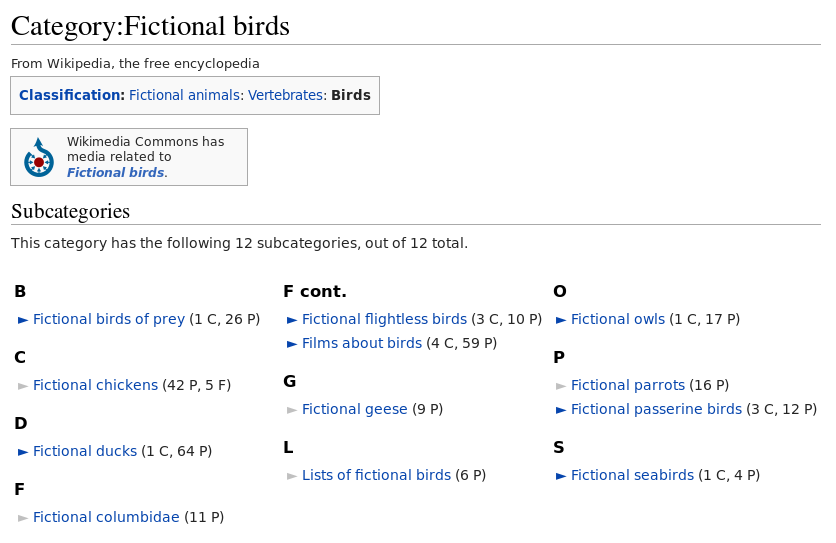
\includegraphics[width=\textwidth]{Chapters/Implementation/Fictional_birds_2}
\caption{The subcategories of the category \emph{Fictional birds} and how its subcategories are sorted based on the defined sortkey instead of the category title }
\label{fig:fictionalbirds}
\end{figure}

%This part of the \texttt{INSERT} statements means that the category \emph{fictional ducks} is both a subcategory of the category \emph{Fictional birds} and the category \emph{ducks}, hence the \texttt{INSERT} statement results in two links, one from \emph{fictional birds} to \emph{fictional ducks} and one from \emph{ducs} to \emph{fictional ducks}.

After processing all titles, they are sorted into two files depending; one for links between categories and one for links between categories and articles. These files are needed for creating the structure for finding full paths of all Wikipedia articles. 

%After the file \texttt{enwiki-latest-categorylinks.sql.gz} was split into two files where the first one contained all links between categories and the second file contained all links between categories and articles. 


\subsubsection{Creating the Category graph}
A category graph is a way of representing links between categories i.e., what categories we can reach from a given category. The file containing all links between categories can be used to create such a graph. The first step is to find all subcategories of each category and remove duplicate links. This should result in a structure like the one represented in figure \ref{fig:categorystructure}

\begin{figure}
\centering
\begin{subfigure}[b]{0.4\textwidth}
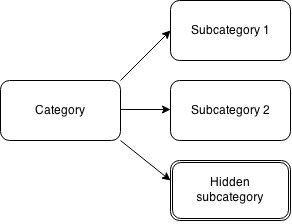
\includegraphics[width=\textwidth]{Chapters/Implementation/category-subcategories}
\caption{The structure where each category knows its subcategories}
\label{fig:categorystructure}
\end{subfigure}
\begin{subfigure}[b]{0.4\textwidth}
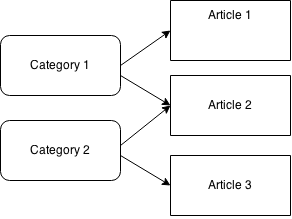
\includegraphics[width=\textwidth]{Chapters/Implementation/categories-articles}
\caption{The structure where each category know the title of its articles}
\label{fig:catartstructure}
\end{subfigure}
\caption[The representation of the Wikipedia structure]{Combined this is the structure needed to represent the Wikipedia's underlying category structure as a graph}
\end{figure}


\subsubsection{Creating the Article graph}
It is also relevant to create a system of all the articles and their most describing categories. The file containing all links between categories and their articles can be used to create a structure where each category knows its articles. Figure \ref{fig:catartstructure} shows an example of how this structure should be represented. Early in this process is it relevant to remove all articles where the titles is only a number, which was found to be  23 227 articles. Number of article links are therefore removed as seen in table \ref{tab:withoutnumber}

\begin{table}[h]
\centering
\begin{tabular}{c|c}
\textbf{W/ Number Articles} & \textbf{W/o Number Articles}  \\ \hline
 3 152 873 & 3 145 455
\end{tabular}
\caption[Number of links without number articles]{Number of links between categories and articles removed when articles only containing numbers are disregarded}
\label{tab:withoutnumber}
\end{table}


% 23227